\documentclass[c,12pt]{beamer}
 \usepackage[T1]{fontenc} 
 \usepackage[utf8]{inputenc}
 \usepackage[french]{babel}
 \selectlanguage{french}
 \usetheme{Warsaw}
 \usepackage{pslatex}
 \usepackage{graphics}
\usepackage{amsfonts}
\usepackage{graphicx}
\usepackage{stmaryrd}
\usepackage{nccmath}
\usepackage{subfigure}
\usepackage{color}

\newcommand{\A}[0]{{\cal A}}
\newcommand{\C}[0]{{\cal C}}
\newcommand{\I}[0]{\cal I}
\newcommand{\se}[1]{\medbreak \medbreak \section*{#1}}
\newcommand{\sse}[1]{\medbreak \subsection*{#1}}
\newcommand{\ssse}[1]{\subsubsection*{#1}}
\newcommand{\Def}[0]{\ssse{Définition}}
\newcommand{\The}[0]{\ssse{Théorème}}
\newcommand{\Pro}[0]{\ssse{Propriété}}
\newcommand{\mb}[1]{\mathbb{#1}}
\newcommand{\Exo}[1]{\sse{Exercice #1}}
\newcommand{\Que}[1]{\ssse{Question #1}}
\newcommand{\ssi}[0]{\Leftrightarrow}
\newcommand{\ra}[0]{\rightarrow}
\newcommand{\Ra}[0]{\Rightarrow}
\newcommand{\la}[0]{\leftarrow}
\newcommand{\La}[0]{\Leftarrow}
\newcommand{\llb}[0]{\llbracket}
\newcommand{\rrb}[0]{\rrbracket}
\newcommand{\dd}[0]{\txt{d}}
\newcommand{\dr}[0]{\partial}
\newcommand{\txt}[1]{\textrm{#1}}
\newcommand{\ol}[1]{\overline{#1}}
\newcommand{\ul}[1]{\underline{#1}}
\newcommand{\abs}[1]{|#1|}
\newcommand{\iso}[0]{\simeq}
\renewcommand{\P}[0]{\cal P}
\newcommand{\Fo}[0]{{\cal F}_0}
\newcommand{\w}[0]{\omega}
\newcommand{\mo}[0]{\models}
\newcommand{\blo}[2]{\begin{block}{#1} #2 \end{block}}
\newcommand{\cols}[1]{\begin{columns}#1\end{columns}}
\newcommand{\col}[2]{\begin{column}{#1}#2\end{column}}
\newcommand{\fig}[3]{\begin{figure} \includegraphics[scale = #1]{#2}\caption{#3}\end{figure}}
\newcommand{\image}[2]{\begin{figure} \includegraphics[scale = #1]{#2}\end{figure}}
\newcommand{\gray}{\textcolor{gray}}


\newcommand{\matrice}[1]{\left(\begin{matrix} #1 \end{matrix}\right)}
\newcommand{\subfig}[1]{\subfigure{\includegraphics[width=40mm]{#1}}}
\newcommand{\Arrow}{{ \raisebox{10\height}{\scalebox{1}{$\longrightarrow$}}}}
\newcommand{\arrow}{{\raisebox{15\height}{\scalebox{1}{$\longrightarrow$}}}}

\newcommand{\fram}[2]{\begin{frame} \frametitle{#1} #2 \end{frame}}

%\usepackage[french,onelanguage]{algorithm2e}
%\usepackage{algorithmique}

\title{Échantillonnage irrégulier par une homographie}
\subtitle{Encadré par Jean-Michel Morel et Enric Meinhardt-Llopis}
 \author{S. Barazer, J.-T. De La Roche Saint-André, H. Moeneclaey, S. Rakotonirina--Ricquebourg}
 \date{30 Juin 2015}

 \AtBeginSection[]{
  \begin{frame}{Sommaire}
  \small \tableofcontents[currentsection, hideothersubsections]
  \end{frame} 
}

\begin{document}
 
\maketitle

 %introduction by shmuel
  \section{Qu'est-ce qu'une homographie ?}
  \begin{frame}
  \frametitle{Position du problème}
   \small{Formule générale : $H : (x,y)\mapsto \left(\frac{ax+by+p}{rx+sy+t},\frac{cx+dy+q}{rx+sy+t}\right)$ telle que $img_f(x,y)=img(H(x,y))$}
   \begin{figure}
    \centering
    \subfig{BriquesOriginal.png}
    \arrow
    \subfig{BriquesTransformed.png}
    \caption{Effet d'une homographie}
   \end{figure}
  \end{frame}
  \begin{frame}
    \frametitle{Position du problème}
   \small{Formule générale : $H : (x,y)\mapsto \left(\frac{ax+by+p}{rx+sy+t},\frac{cx+dy+q}{rx+sy+t}\right)$ telle que $img_f(x,y)=img(H(x,y))$}
   \begin{figure}
    \centering
    \subfig{BriquesOriginal.png}
    \arrow
    \subfig{BriquesTransformedExtended.png}
    \caption{Effet d'une homographie prolongée périodiquement}
   \end{figure}
  \end{frame}



 
 \fram{Méthode naïve}{
 	\cols{
 		\col{5cm}{$img_f(x,y)=img(H(x,y))$ 
			\medbreak
			On applique naïvement cette formule : valeur du pixel le plus proche
			\fig{0.25}{imageproque.jpg}{Pourquoi cela ne fonctionne pas}
		}
		\col{5cm}{
			\fig{0.3}{barbara}{Une application naïve sur une image périodique}
		}
 	}
 }
 %Et slide sur la zone à intégrer
 
 
 %moi+jeanthomas
 \section{Méthodes actuelles}
 
 \subsection{Mipmap}
 
\fram{Approximation à l'aide du Mipmap}{
	\cols{
		\col{5cm}{
			Présenté par Williams, \underline{Pyramidal parametrics}, 1983 %le mettre en bas de page ?
 %$\ra$ Précalcul de zones%eventuellemnt image des parallélogramme
			\image{0.3}{approx.jpg}
			\blo{Problèmes}
			{
				\begin{itemize}
				\item Fonctions de distance
				\item Construction du Mipmap
				\end{itemize}
			}
			-> variante anisotropique : Ripmap
		}
		\col{5cm}{\fig{0.35}{MipMap_real}{Un exemple de Mipmap}}
	}
}
 
 
 \fram{L'interpolation trilinéaire}{\image{0.5}{intertri.jpg}}
 
     
     
     
    
     
     
     
     
     
     
     
     
     
     
\section{Méthode géométrique}
 
 \subsection{Décomposition d'une homographie}

  \subsubsection{Homographie unidirectionnelle}

  \begin{frame}{Homographie unidirectionnelle}
   \begin{block}{Définition}
    Une homographie unidirectionnelle est une homographie de la forme
    \[\tilde H : (x,y) \mapsto \left(\frac{ax+\gray{by}+p}{rx+\gray{sy}+t},\frac{\gray{cx}+dy+q}{rx+\gray{sy}+t}\right)\]
    avec $b=c=s=0$
   \end{block}
   \begin{block}{Théorème}
    Pour toute homographie $H$, il existe $T$ une translation, $R_\phi$ et $R_\psi$ des rotations et $\tilde H$ une homographie unidirectionnelle telle que
    \[H = T R_\phi \tilde H R_\psi\]
   \end{block}
  \end{frame}
  

  
\subsubsection{Visualisation de la décomposition}

  \begin{frame}{Décomposition géométrique d'une homographie}
  \begin{figure}
   \centering
   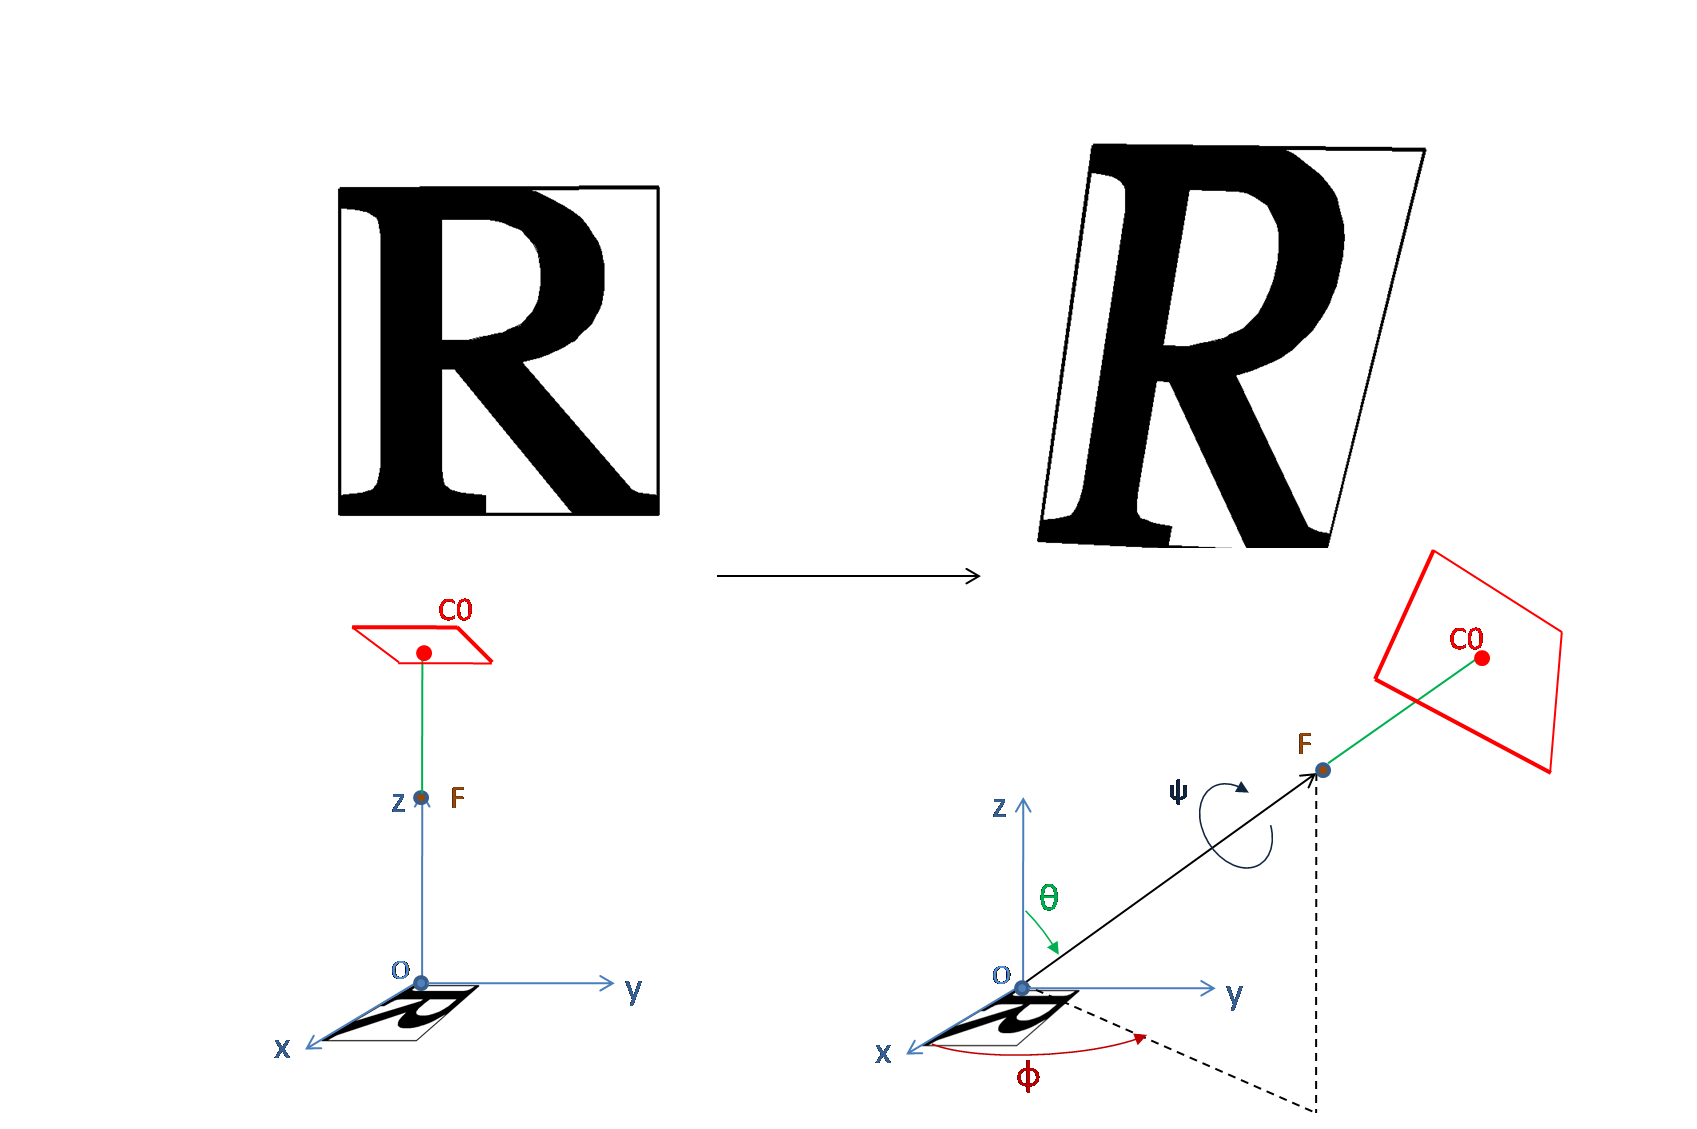
\includegraphics[width=100mm]{beamer_decompo_all.png}
   \caption{Homographie quelconque vue comme un mouvement de caméra}
  \end{figure}
  \end{frame}

  \begin{frame}{Décomposition géométrique d'une homographie}
  \begin{figure}
   \centering
   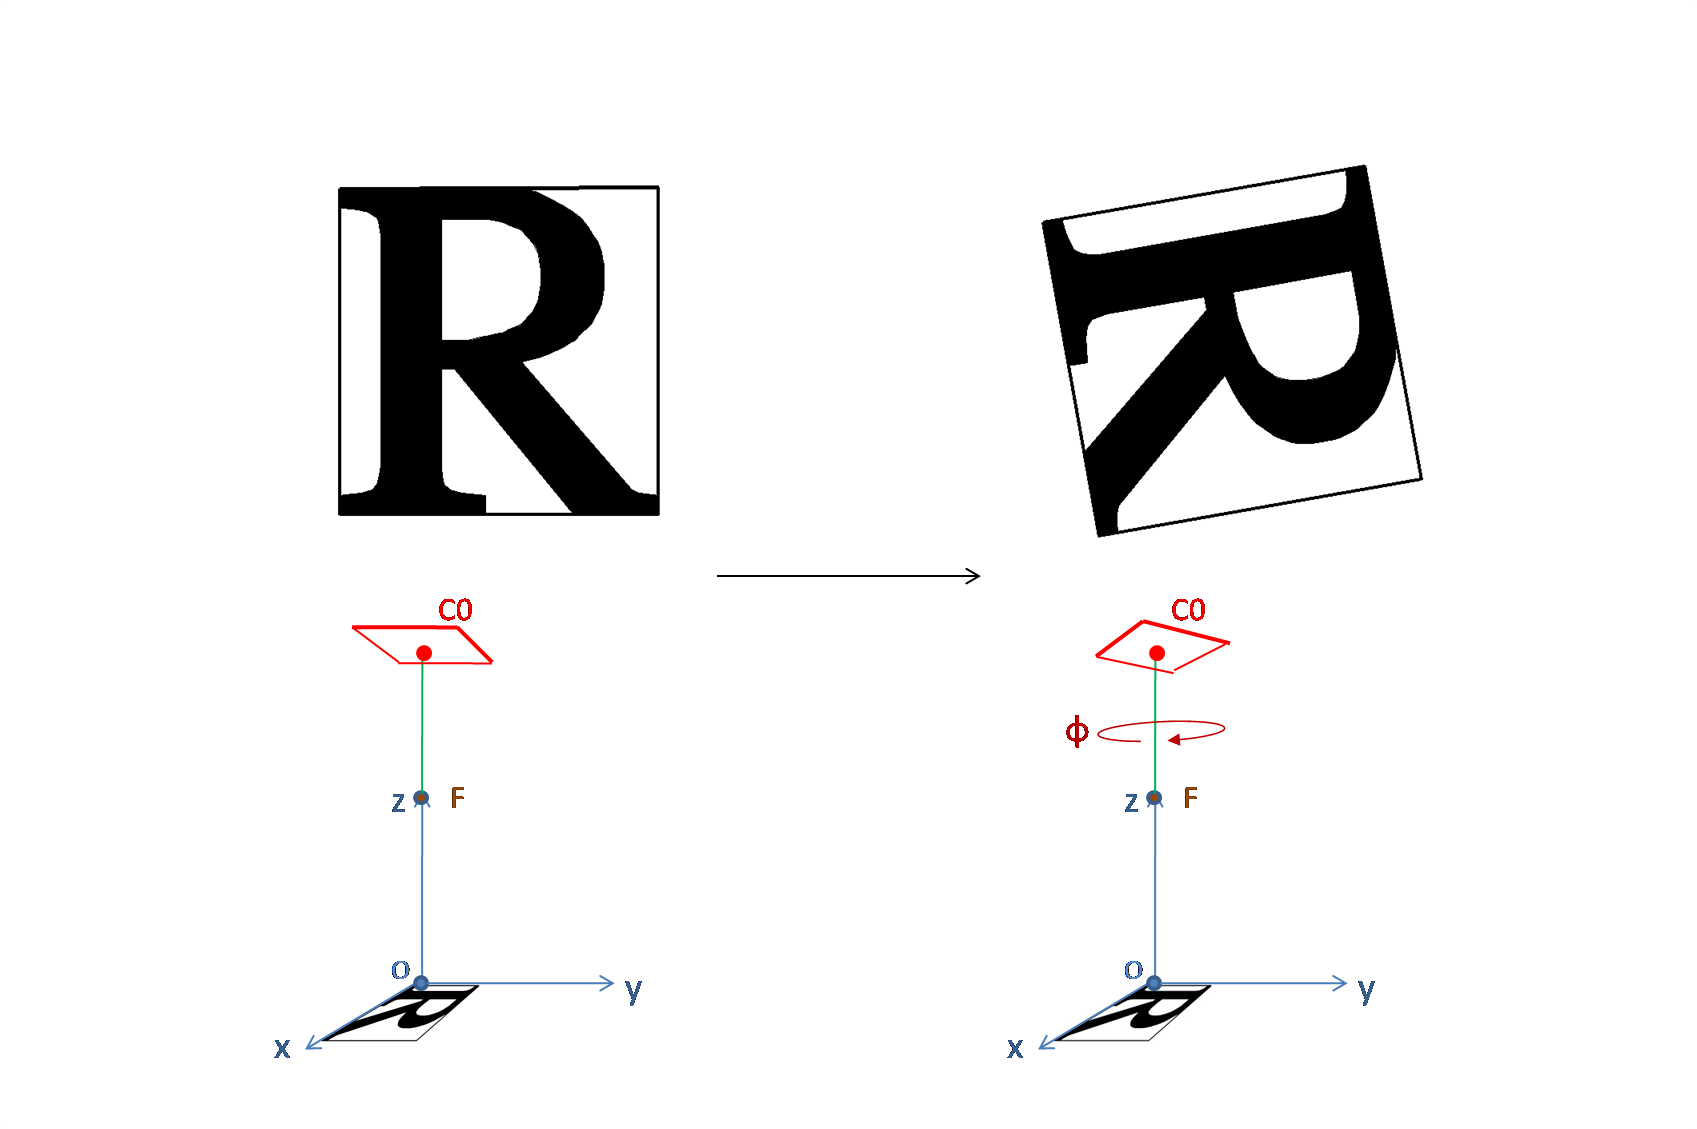
\includegraphics[width=100mm]{beamer_decompo1_rotation_phi.png}
   \caption{Première rotation}
  \end{figure}
  \end{frame}

  \begin{frame}{Décomposition géométrique d'une homographie}
  \begin{figure}
   \centering
   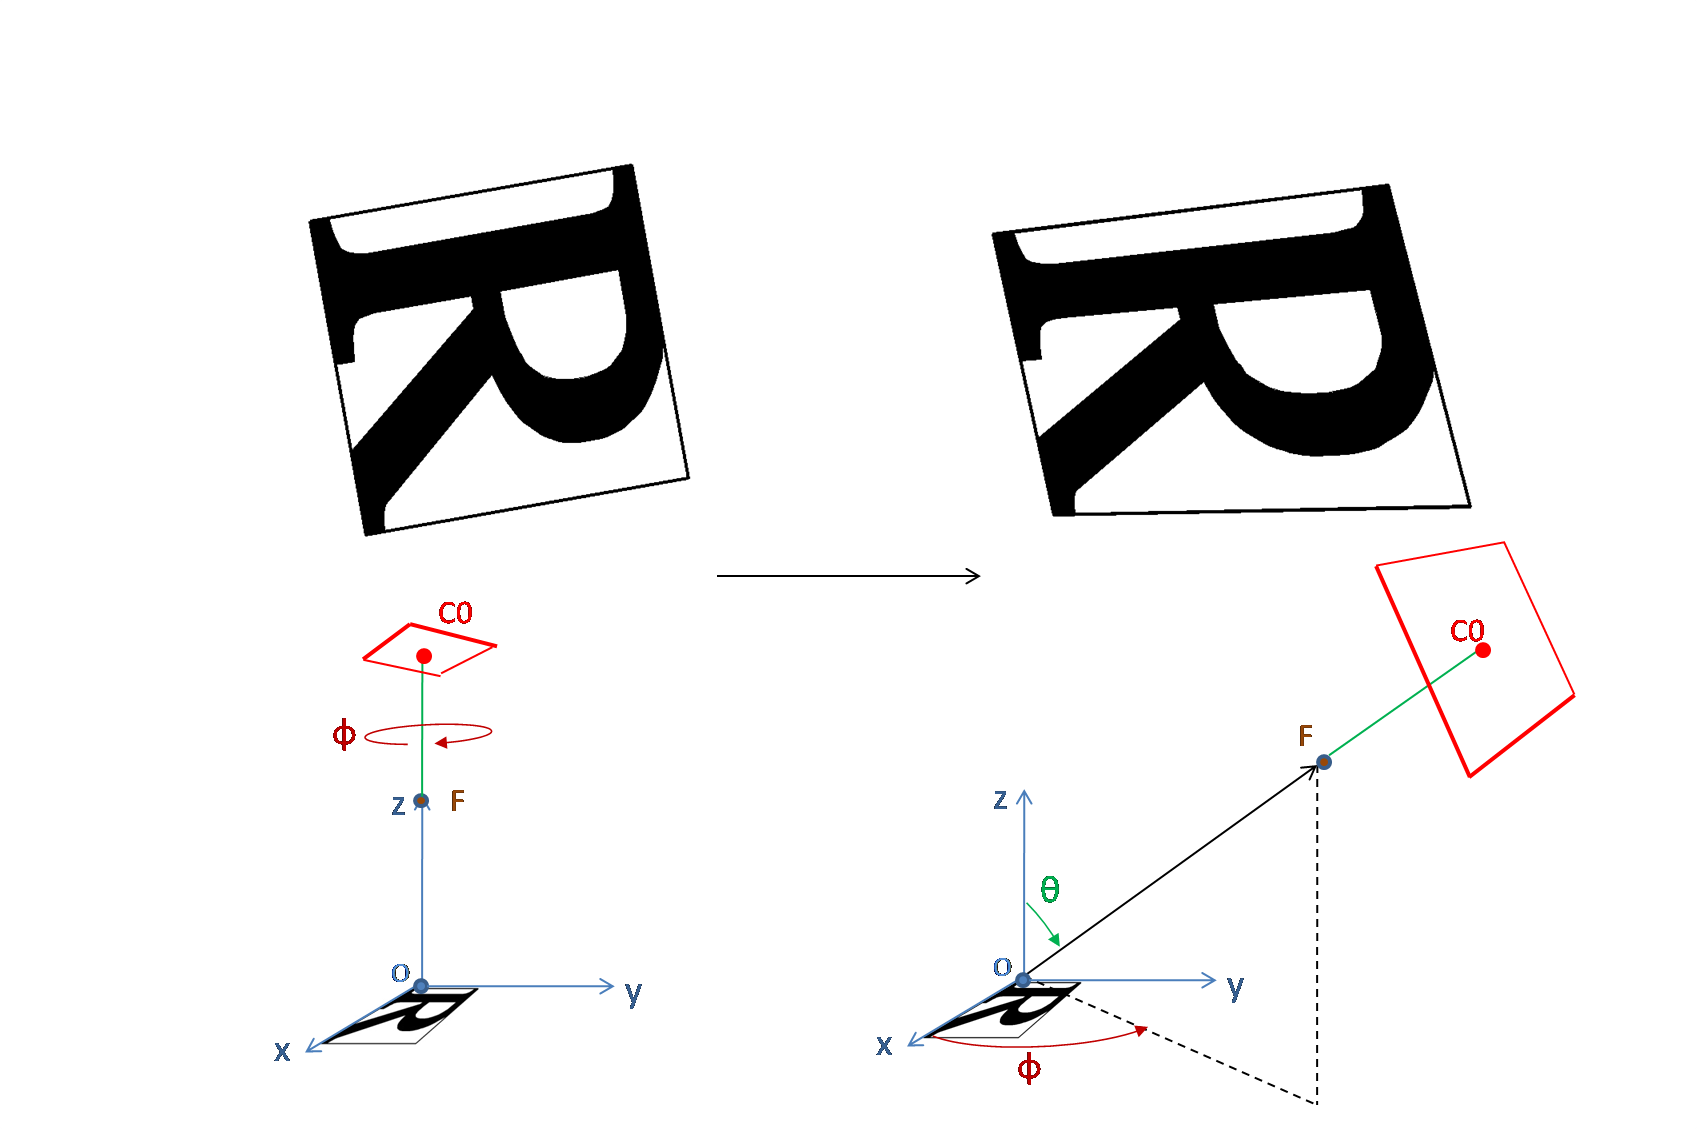
\includegraphics[width=100mm]{beamer_decompo2_homo_part.png}
   \caption{Homographie unidirectionnelle}
  \end{figure}
  \end{frame}

  \begin{frame}{Décomposition géométrique d'une homographie}
  \begin{figure}
   \centering
   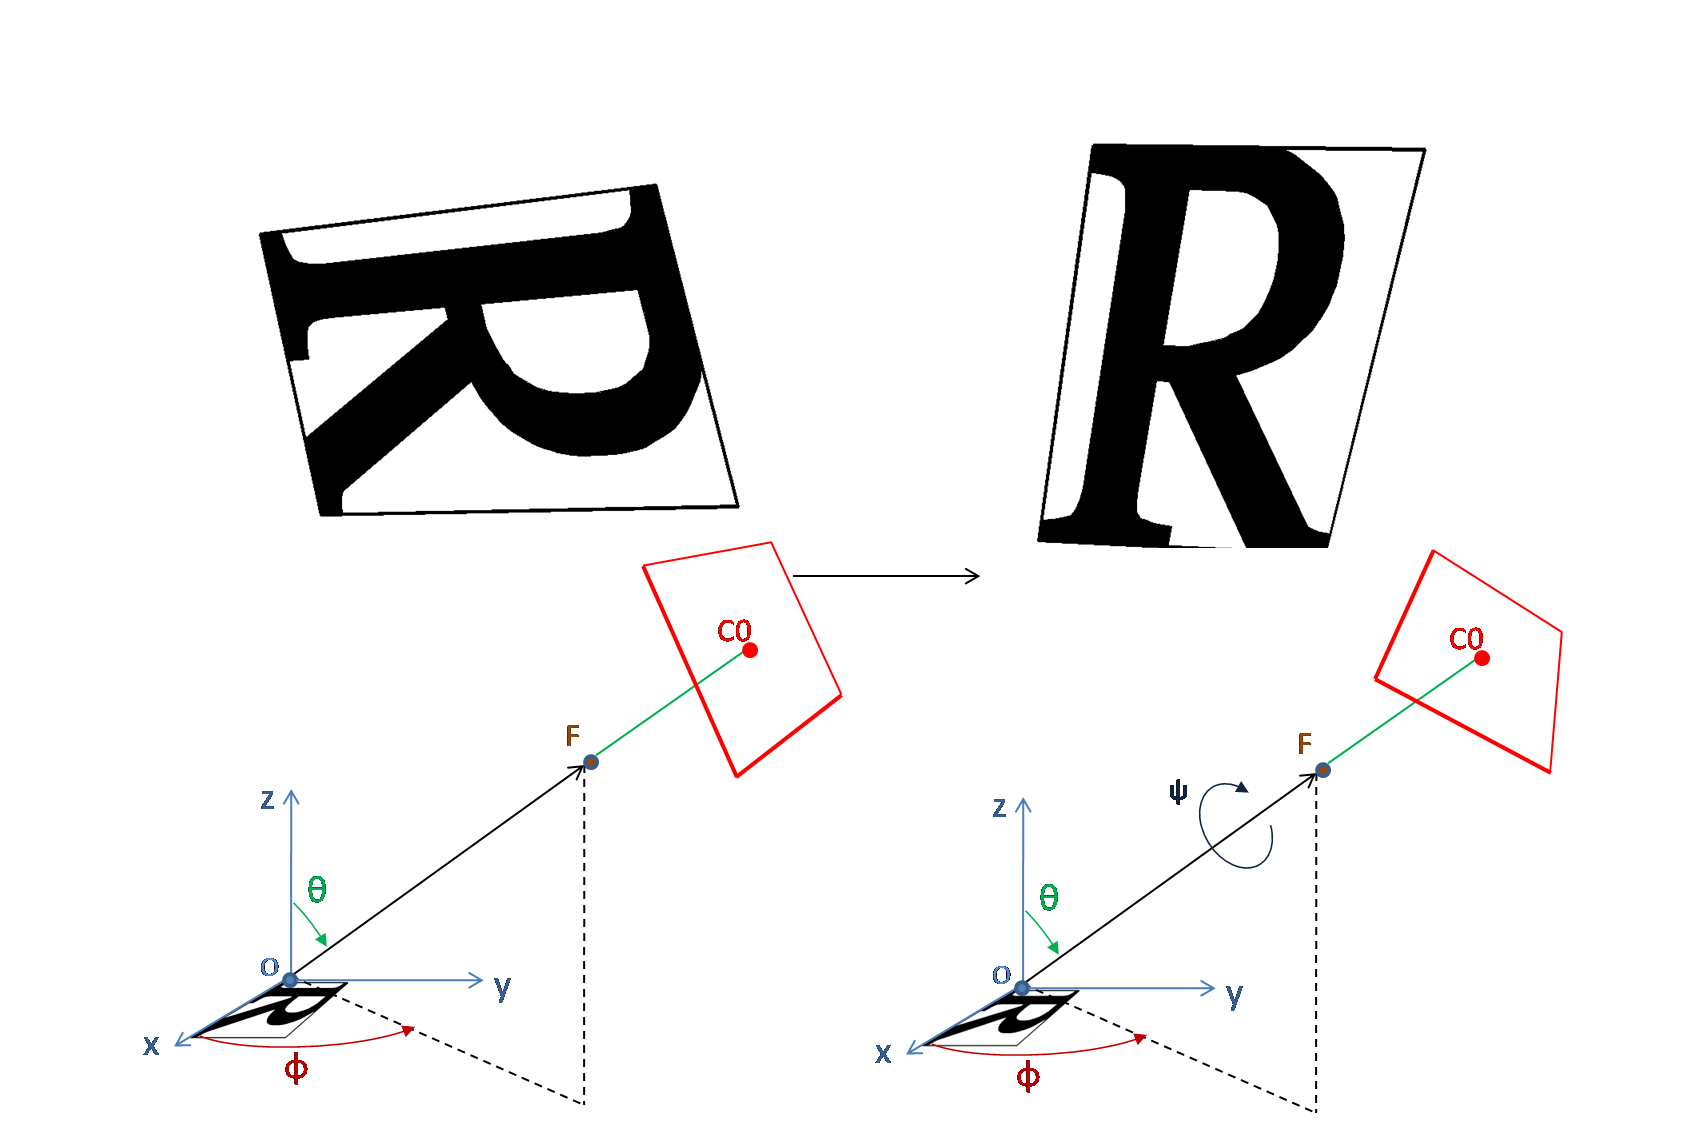
\includegraphics[width=100mm]{beamer_decompo3_rotation_psi.png}
   \caption{Seconde rotation}
  \end{figure}
  \end{frame}

  \begin{frame}{Décomposition géométrique d'une homographie}
  \begin{figure}
   \centering
   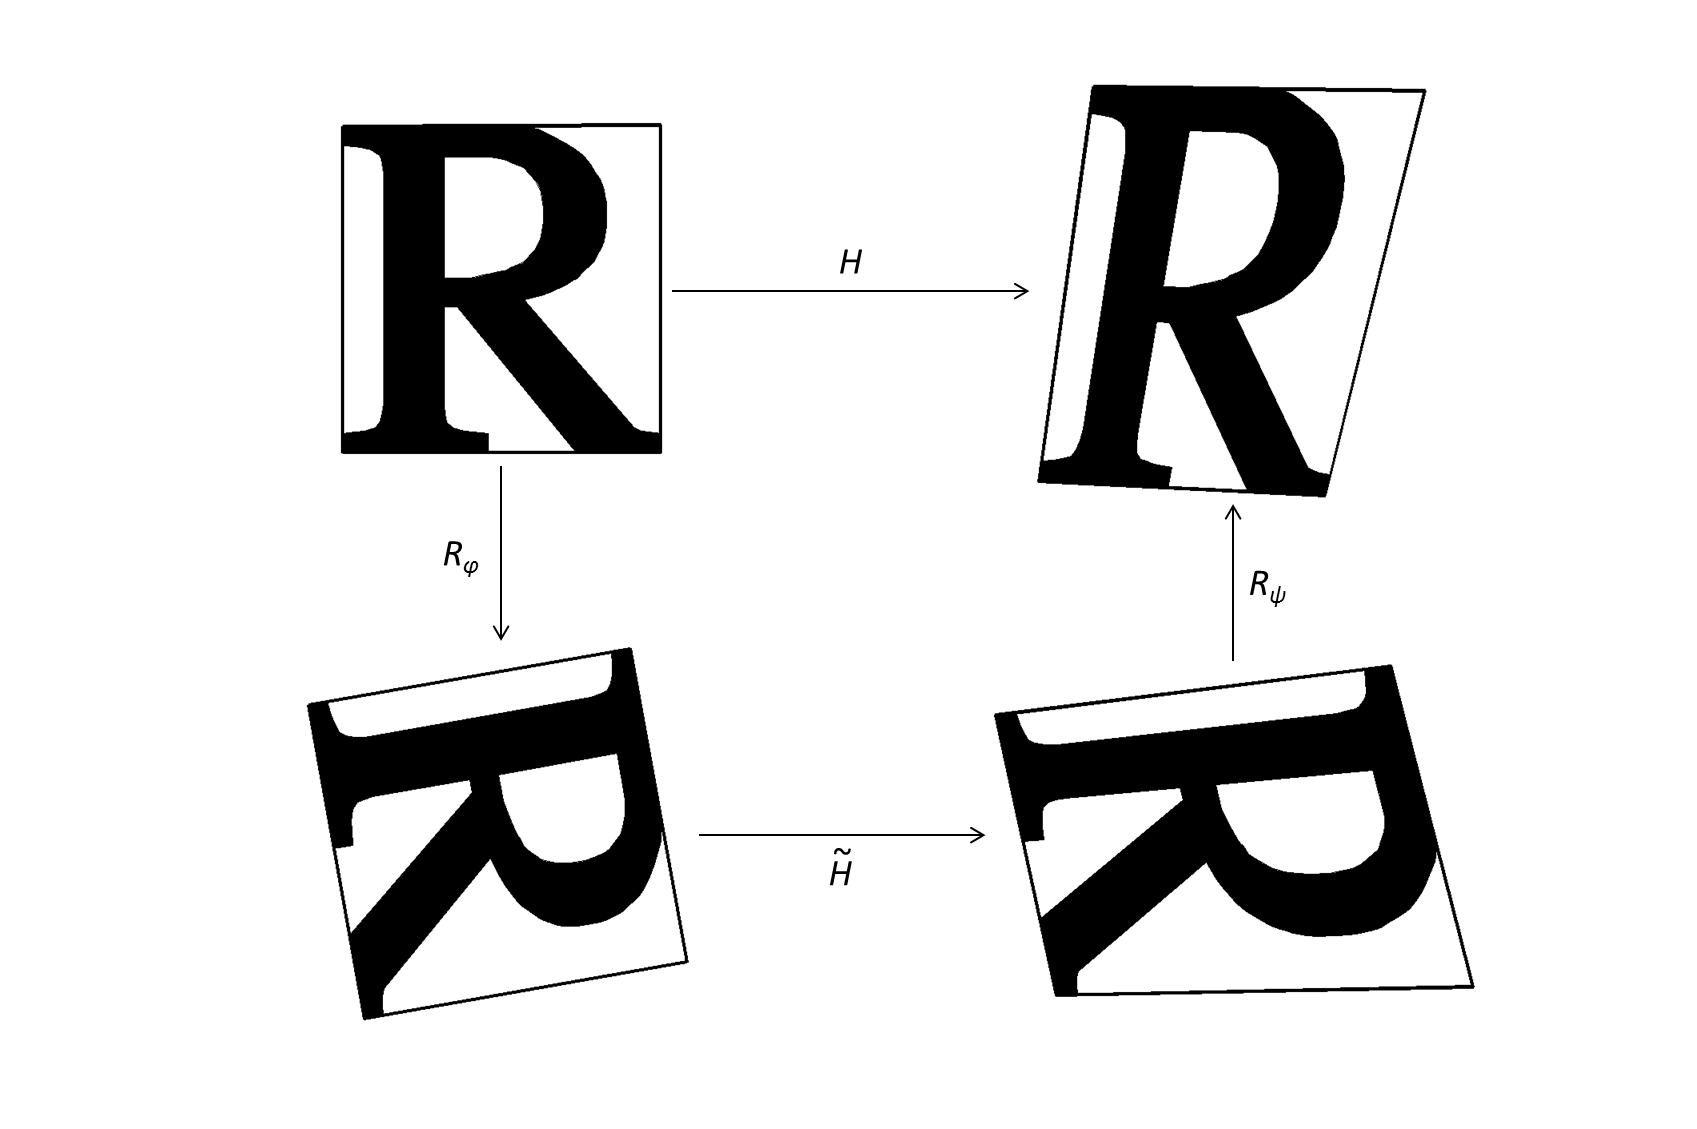
\includegraphics[width=100mm]{beamer_decompo_bilan.png}
   \caption{Décomposition}
  \end{figure}
  \end{frame}

%truc simon a inséréer sur affine




\subsection{Traitement des rotations}
\begin{frame}{Etude des rotations}

\begin{figure}
\centering
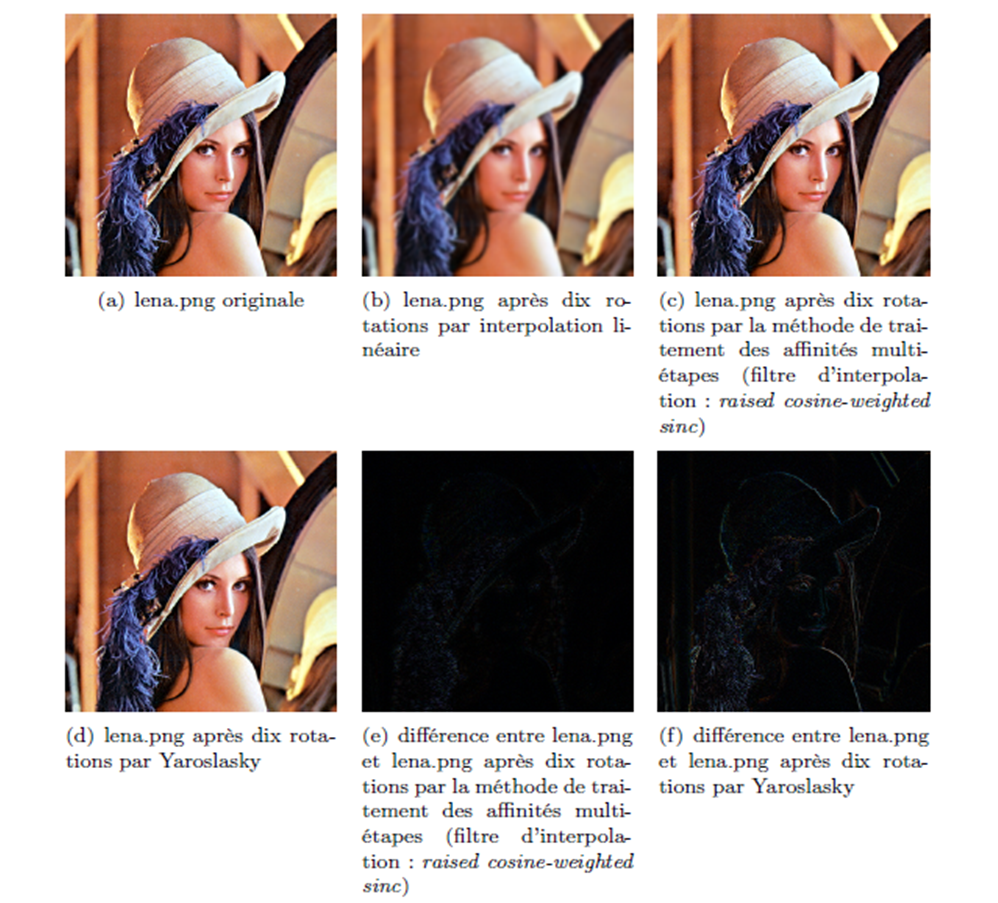
\includegraphics[width=6cm]{rotation_all.png}
\caption{Comparaison des rotations}
\end{figure}

\end{frame}
\begin{frame}{Etude des \emph{shears} (cisaillement)}

Introduit dans Szeliski, \underline{High quality multi-pass image resampling} en 2010. %mettre en bas de page ?

\begin{itemize}
\item minimiser l'aliasing sans filtrage préalable.
\end{itemize}

\begin{columns}
\begin{column}{5cm}

\begin{block}{Algorithme pour un \emph{shear}}

$\ra$ trois étapes :

\begin{itemize}
\item zoom avant
\item \emph{shear}
\item filtrage passe bas et zoom arrière
\end{itemize}

\end{block}
  
 \end{column}

\begin{column}{5cm}

\begin{figure}
\centering

\includegraphics[width=4cm]{dragonshear.jpg}
\caption{\emph{Shear} horizontal}
%\caption{\emph{Shear} horizontal de matrice $\begin{pmatrix}
%a_0 & a_1\\ 0 & 1
%\end{pmatrix}$ \tiny{(où $img_f[i][j] = \sum_k h\left(\frac{a_0i+a_1j-k}{s}\right)img[k][j]$, $h$ un noyau de convolution)}\red{slide spécial pour chaque $\mathcal R$ ?}}
\end{figure}

\end{column}
\end{columns}
\end{frame}



\begin{frame}{Illustration de la méthode dans le domaine de Fourier }

\begin{figure}
\centering
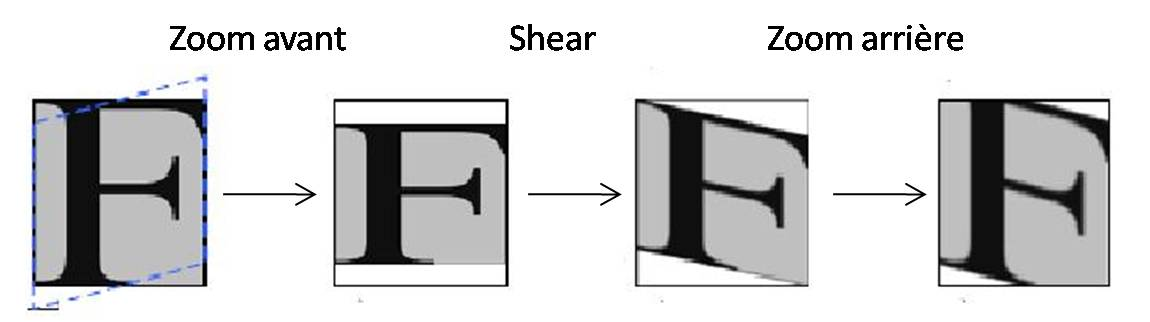
\includegraphics[width=7cm]{fourier1.jpg}
\caption{Méthode de Szeliski}
\end{figure}

\begin{columns}
\begin{column}{4cm}

\begin{figure}
\centering
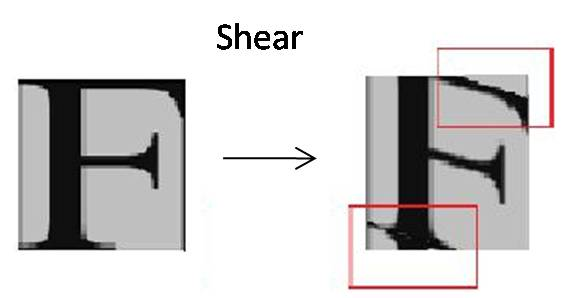
\includegraphics[width=3cm]{fourier2.jpg}
\caption{Méthode naïve}
\end{figure}

%On observe un repliement du spectre ce qui provoque de l'aliasing.

\end{column}

\begin{column}{6cm}

\begin{figure}
\centering
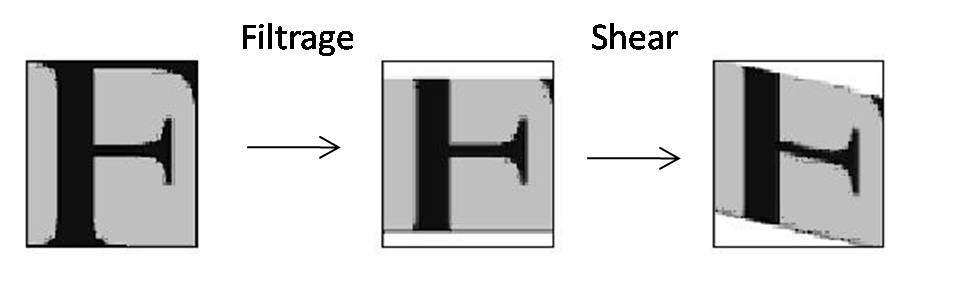
\includegraphics[width=5cm]{fourier3.jpg}
\caption{Méthode par filtrage}
\end{figure}

%Une partie du spectre a été perdue lors du filtrage

\end{column}
\end{columns}

\end{frame}




\begin{frame}{Méthode finale pour les affinités}
%rajouter qqvh....
\begin{itemize}
\item Affinités $\ra$ composée de deux \emph{shears}.
%$A=S_v \circ S_h$
\item translations sur les lignes et les colonnes.
%\item On réutilise la méthode développée pour les \emph{shears}.
%\item L'algorithme final se décompose en 6 étapes que l'on peut réduire à  4.
\end{itemize}

\begin{block}{Schémas de l'algorithme final}

\begin{itemize}
\item Zoom avant vertical
\item \emph{Shear} horizontal
\item \emph{Shear} vertical
\item Filtrage passe bas et zoom arrière horizontal
\end{itemize}

\end{block}

\end{frame}




 \subsection{Traitement des homographies unidirectionnelles}
     
     
     
    
     
     
     
     
     
     
     
     
     
     
\section{Expériences et résultats}
     

\fram{}{\fig{0.35}{img_geo_5.png}{Homographie 1 à l'aide de la décomposition}}
\fram{}{\fig{0.35}{img_ripmap_5.png}{Homographie 1 à l'aide du Ripmap}}

\fram{}{\fig{1.5}{img_geo_moustache.png}{Homographie 1 à l'aide de la décomposition (détail)}}
\fram{}{\fig{1.5}{img_ripmap_moustache.png}{Homographie 1 à l'aide du Ripmap (détail)}}

\fram{}{\fig{0.35}{img_f_2.png}{Homographie 1 à l'aide de la décomposition}}
\fram{}{\fig{0.35}{img_ripmap_2.png}{Homographie 1 à l'aide du Ripmap}}



 
% \fram{Schema pour le ripmap}{\image{0.5}{pbripmap}}
 
\end{document}
